%!TEX root = ../../super_main.tex

\chapter{Architecture}
\label{cha:architecture}

We will in this chapter introduce the architecture that will facilitate a solution corresponding to the vision in \secref{sec:vision}. An overview of the architecture are shown in \figref{fig:system_architecture}, which show that we have two main component, namely a server and a client. The overall purpose and a brief description of these, the communication between them, and their subcomponents will be covered in this chapter. A more detailed description of the features that they provide will be covered in the following chapters.

\begin{figure}[!htbp]
    \centering
    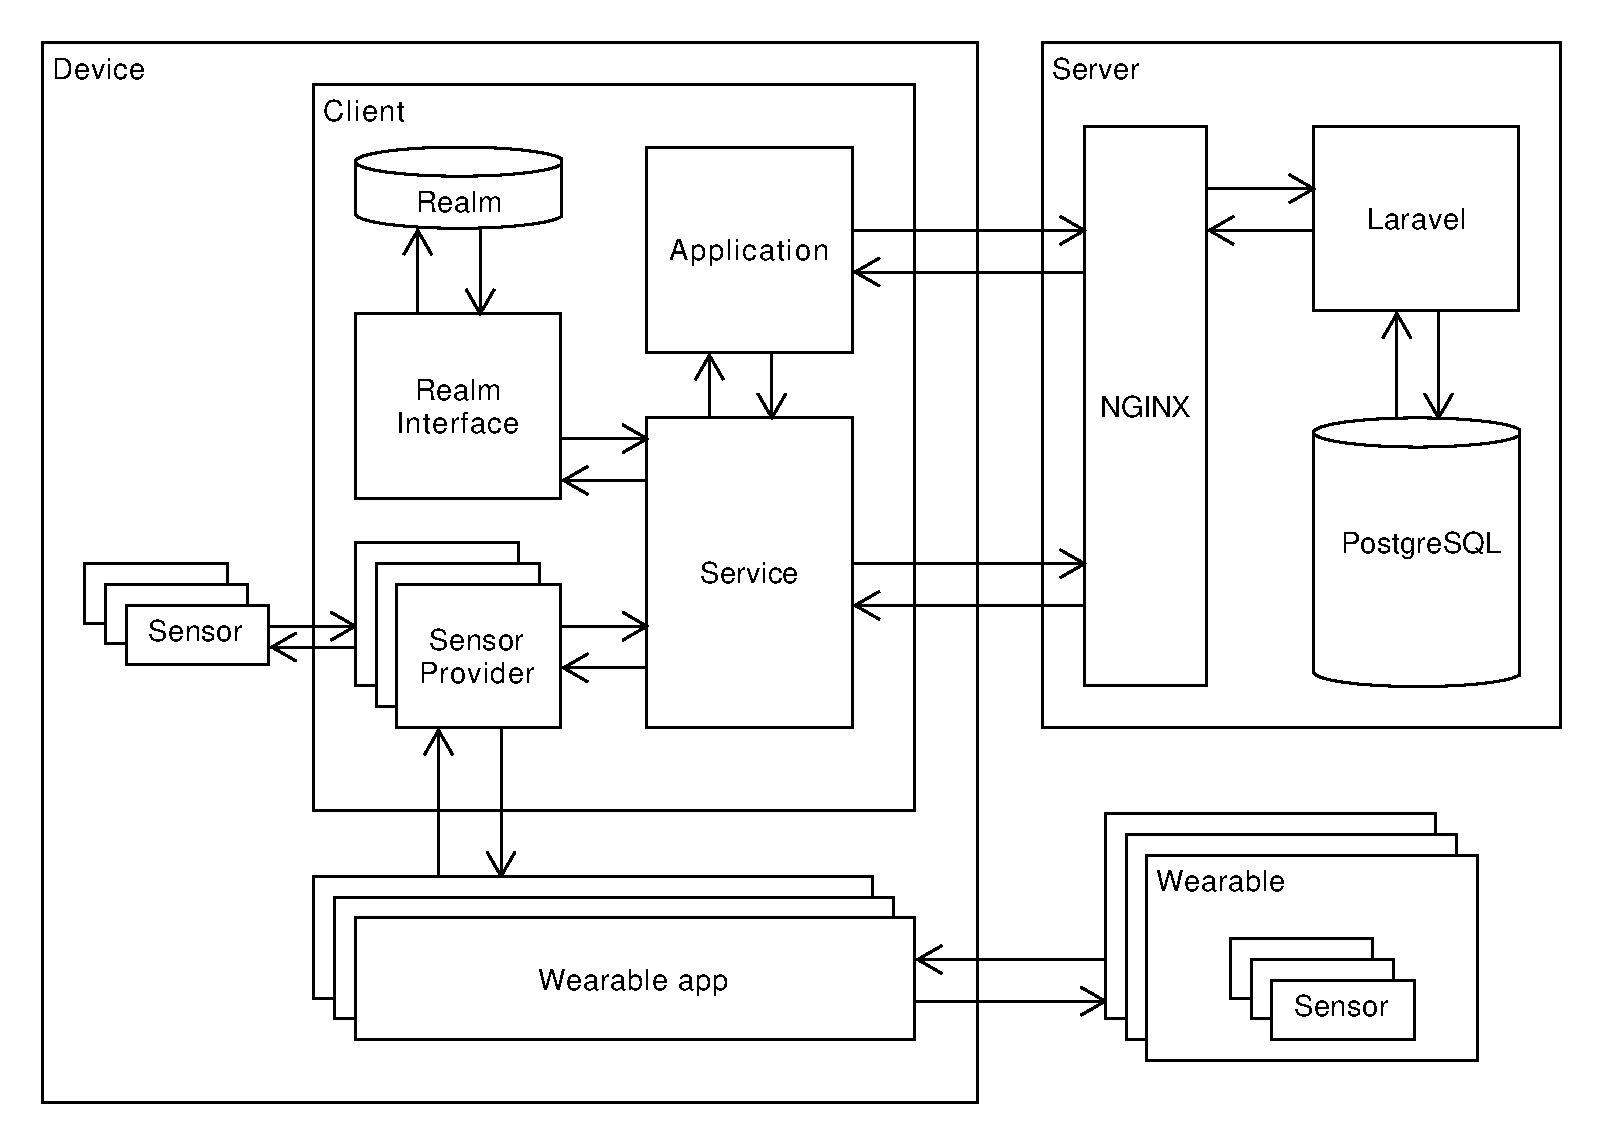
\includegraphics[width=\textwidth]{graphic/architecture/architecture.pdf}
    \caption{An abstract overview of the overall system architecture.}
    \label{fig:system_architecture}
\end{figure}
\FloatBarrier

%!TEX root = ../../super_main.tex
\section{Server}
The server provides the interface for the customers of the system, the ones in need of campaigns. Besides allowing the customers to specify campaigns the, server is also responsible for handling the upstream of snapshots from the devices of the participants. Meaning that the server has both a application programming interface (API) \todo{check if this is the first place we mention API} and a graphical user interface (GUI) \todo{check if this is the first place we mention GUI} for the customers. The server runs a web server technology called NGINX which handles the network communication using the hyper text transfer protocol (HTTP) \todo{check if this is the first place we mention HTTP} and allows for using transport layer security (TLS) \todo{check if this is the first place we mention TLS}. Furthermore this web server is also able to communicate with the underlying operating system to be able to read files from disk and interpret PHP code.
\\\\
With these features of NGINX the server is now able to facilitate the web framework Laravel. This framework builds on the model-view-controller (MVC) pattern. This allows us to route incoming requests and handle them as both application request but also as user requests. 

\todo[inline]{Snak om PostgreSQL}

%!TEX root = ../../super_main.tex

\section{Device}
\label{sec:device}
The device component is the part of the system that should run directly on the smartphone of the participant. This component is responsible for interacting with the participants, gather data from the sensors on the device, and communicating with the other devices in order to get data from wearables. The sensors represent the underlying hardware, and the Wearable Application is the interface from the client application to external wearable sensors, which in our case is the Microsoft Health application that communicates with Microsoft Band 2 we have implemented support for in the system.
\\\\
The client application contains a service component that is the main controller of the system client application. This service runs independently in the background at all times, and is the part of the system on a device that communicates with the different sensor providers, and also uploads the collected snapshots to the server. Furthermore it is also responsible for prompting the participants to answer the questionnaires. This service is completely detached from the interfaces, since it needs to ensure guarantees in respect to the real time aspects of gathering the sensor data.
\\\\
The UI components consists of two interfaces, a settings interface and a questionnaire interface. The settings interface allows for the participant to browse details and join campaigns. Furthermore, it also has some communication with the web server where it fetches the specifications of campaigns, and reports back to the server which campaigns the participants has joined. The questionnaire interface is a series of user inputs where the participants can provide answers for the questions of a questionnaire. This interface is prompted to the user by using notifications, which are sent by the service for every snapshot, in order to obtain labels on the data if possible.
\\\\
The service component is also in need of some persistent storage on the device, to ensure that it can store gathered snapshots, so that it can upload the data using best practices in regards of power consumption and robustness as described in \secref{sec:general_strategies}. For this reason the application has a storage module where we utilize a library called \mono{realm}, which will be further describe in \secref{sub:local_storage}.
\\\\
Lastly the service component is heavily dependent on the sensor providers, which are providers that abstracts various types of sensors, for example hardware sensors on the device, software sensors, and external sensors from wearable and so on. From the service point of view, it only needs to manage the specification of campaigns and request the data from these providers accordingly before it stores the data that has been gathered from these providers on the device. The controller of the service assumes that the interface of these providers guarantees the amount of data requested and that they keep their deadlines in regards to timing of measurements.
